\documentclass{article}
\usepackage{graphicx}
\usepackage{float}
\usepackage[center]{caption}
\usepackage{multicol}
\usepackage{multirow}
\usepackage{listings}
\usepackage{color}
\usepackage{pgfplotstable, booktabs}
\setlength{\abovecaptionskip}{2pt plus 3pt minus 2pt} 
\definecolor{dkgreen}{rgb}{0,0.6,0}
\definecolor{gray}{rgb}{0.5,0.5,0.5}
\definecolor{mauve}{rgb}{0.58,0,0.82}
\usepackage[a4paper, total={6in, 8in}]{geometry}
\lstset{frame=tb,
  aboveskip=3mm,
  belowskip=3mm,
  showstringspaces=false,
  columns=flexible,
  basicstyle={\small\ttfamily},
  numbers=none,
  numberstyle=\tiny\color{gray},
  keywordstyle=\color{blue},
  commentstyle=\color{dkgreen},
  stringstyle=\color{mauve},
  breaklines=true,
  breakatwhitespace=true,
  tabsize=3
}
\graphicspath{ {COMP_PROJECT/} }
\begin{document}
\title{Molecular Dynamics Simulation: \break Lennard-Jones Cluster Collision}
\author{C.T.Hutchinson}
\maketitle

\newpage




\begin{abstract}
The use and design of a simple Molecular Dynamics program written in Python 3 is demonstrated to model the collision of two Lennard-Jones clusters. The system is evolved in time by integration of Newton's equations of motion via the Velocity Verlet algorithm. The two clusters are found to coalesce within 50 nanoseconds when the time-step is set to 1 picosecond, and initialised at distance 5 and incoming velocity 1e8.
\end{abstract}
\begin{multicols}{2}
\part{Introduction}
In this paper we model the collision of two Lennard-Jones clusters in dimensionless units through a Molecular Dynamics simulation code. Two clusters of particle size 70 and 77 \cite{doye} are used in the simulation, with one arbitrarily centred at the origin of the co-ordinate system. The other cluster is displaced some distance in the x-axis direction, with an initial velocity chosen by the user. A user assigned initial separation can be seen below in the 3D plot shown in Figure 1.
\begin{figure}[H]
\center
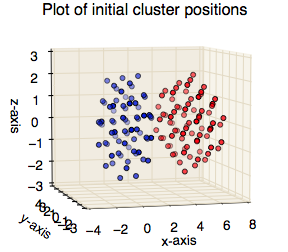
\includegraphics[height=5cm,width=6cm]{init_cluster_pos}
\captionsetup{font=footnotesize, justification=centering,singlelinecheck=false}
\caption{A plot of the initial positions of the two Lennard-Jones clusters.}	
\fontsize 12
\end{figure}


 The simulation is then allowed to proceed during a predetermined time interval of 50 nanoseconds with the force and energy at each particle calculated for each time step of 1 femtosecond \cite{time-step}, according to the Lennard-Jones potential: 
 \[U = 4 \epsilon \Big[ \Big(\frac{\sigma}r\Big)^{12} - \Big(\frac{\sigma}r \Big)^6 \Big]\]

\begin{flushleft}
 With $\epsilon$ the potential well depth, $\sigma$ the distance at which the inter-particle potential is zero and \textit{r} the distance between the two particles.
 \end{flushleft}
 
 In reduced units: \[\sigma,\epsilon=1\]
 
 And therefore the equation for the Lennard-Jones potential becomes:
 
 \[U = 4\Big[ \Big(\frac{1}r\Big)^{12} - \Big(\frac{1}r \Big)^6 \Big]\]
 
 Knowing the force is the derivative of the potential we can derive an expression for the component of force on each particle in each direction, due to the others. Suppose we wish to calculate the \textit{x}-component of the force \cite{frenkel}:
 \[ F_x(r) = -\frac{\partial U(r)}{\partial{x}}
  = -\Big(\frac{x}{r}\Big) \Big(\frac{\partial U(r)}{\partial r}\Big) \]
  
  Which yields:
  \[F_x(r) = \frac{48x}{r^2} \Big(\frac{1}{r^{12}} - \frac{1}{2} \frac{1}{r^6}\Big) \]
  
  The force for the y and z components are calculated likewise, with the total force being the sum of these components. 
  
The core of the Molecular Dynamics simulation is in evolving the system to observe the dynamics and interactions between the clusters with time. In order to evolve the system we must integrate Newton's equations of motion, achieved in this simulation through the use of the Velocity Verlet algorithm \cite{frenkel}. The Verlet Velocity algorithm makes use of Taylor Expansions of position around (\textit{t+$\Delta$t}) and (\textit{t-$\Delta$t}) to calculate the new position and velocity of each particle at each time-step. \newline Position update:
\[r(t+\Delta t) \approx 2r(t) - t(t-\Delta t) + \frac{f(t)}{m}\Delta t^{2}\]
Velocity update:
\[v(t+\Delta t) = \frac{r(t+\Delta t) - r(t-\Delta t)}{2\Delta t}\]

With \textit{r} the position at a chosen time, \textit{t} the time, \textit{f} the force at a given time \textit{t} and $\Delta$\textit{t} the predefined time-step. 
\newline In conjunction with our previous method of calculating the force according to the Lennard-Jones potential, we are now able to successfully evolve the system and observe the dynamics of the two clusters upon computation.

  Furthermore, the instantaneous temperature at a time \textit{t} can be calculated according to the equipartition theorem \cite{frenkel}.
  \[T(t) = \sum \frac{mv^{2}(t)}{N_f k_b}\]
    Where \textit{k\textsubscript{b}} is the Boltzmann constant, \textit{T(t)} the temperature at time \textit{t}, \textit{m} the mass of the particle, \textit{v} the velocity of the particle at time \textit{t} and \textit{N\textsubscript{f}} the number of degrees of freedom.

\part{Methodology}

The code is composed of two main sections. A section where the required functions for the simulation are defined, and a section where the program variables are input and functions called. The latter section is the core of the program and essentially where the simulation takes place.

The two core functions in the program are the Velocity Verlet algorithm and the force calculation, as discussed in the Introduction, named 
\textit{verlet\_vel} and \textit{get\_force} in the code respectively. Other "housekeeping" functions and additional features are also included in the first section of the code, with each being breifly described below in chronology with appearance in the source code. \newline The first function defined is the \textit{get\_clusters} function which simply reads the co-ordinates of the two clusters from a .dat file, and loads them as two matrices. These two matrices, along with an initial separation and velocity are passed to the next function: \textit{init}, the initialisation function. Upon runtime the values of initial separation and velocity are input by the user. The initialisation function proceeds to stack these two matrices into one, creating the current position matrix: \textit{c\_pos}. The first cluster is set to be stationary, and the second cluster to be some user input distance away, travelling towards the first cluster at the given velocity. Additionally, the \textit{init} function also creates the matrices used for storing the kinetic energy, potential energy and force values, initialising them at zero. These three values are stored in matrices \textit{en\_kin}, \textit{en\_pot} and \textit{frc} respectively. \newline The current position, force and potential energy matrices then proceed into the force calculation, completed by the function: \textit{get\_force}. Here the program loops through each particle, being each row of the matrix, calculating the distance in the \textit{x}, \textit{y} and \textit{z} components. These components are then combined to create a squared distance vector \textit{r\_sqr}, to be compared against the cutoff radius \cite{frenkel}. The cutoff radius is a result of truncation of the Lennard-Jones potential, which is required in order to limit the number of meaningful calculations we make. A truncation of interactions is suitable for a system concerned with short range interactions, one where particles within some cutoff distance \textit{rcut} determine the potential energies. Simple truncation of the Lennard-Jones potential can result in substantial error in some cases, however given our simplified system this form of truncation is tolerable.
  \[
    \ U^{trunc}(r)=\left\{
                \begin{array}{ll}
                  U^{LJ} \qquad r\leq rcut\\
                  0 \qquad \quad r > rcut
                \end{array}
              \right.
  \]
The value of \textit{rcut} given in this simulation is 2.5, which corresponds to a value of $\approx$ 3.82\AA  \cite{ercolessi} . This cutoff radius employed also gives rise to \textit{ecut}, which is the value of potential energy at the cutoff radius \cite{frenkel}:

\[ecut=4 \Bigg( \frac{1}{r_{cut}^{12}} - \frac{1}{r_{cut}^6} \Bigg)\]

If the two particles compared during the force calculation are within the cutoff radius, the force for each component is calculated according to:

\[F_x(r) = \frac{48x}{r^2} \Big(\frac{1}{r^{12}} - \frac{1}{2} \frac{1}{r^6}\Big) \]

as derived in the Introduction, and the force in each component of each particle updated. The force for one particle is updated as the positive value, and the other as the negative value, as:
\[F_{ij} = -F_{ji}\]
The potential energy of the particle is also updated, with each particle sharing the calculated value. The force and potential energy updates can be seen in the code as follows:
\begin{flushleft}
\captionsetup[lstlisting]{position=bottom,font=footnotesize}
\renewcommand{\lstlistingname}{Code}
\begin{lstlisting}
#force update in all cartesian components		
frc[i,0]= frc[i,0]+ff*xr
frc[i,1]= frc[i,1]+ff*yr
frc[i,2]= frc[i,2]+ff*zr
frc[j,0]= frc[j,0]-ff*xr
frc[j,1]= frc[j,1]-ff*yr
frc[j,2]= frc[j,2]-ff*zr
#potential energy update
en_pot[i] = en_pot[i] + 2*(r6i*(r6i-1)-ecut) 
en_pot[j] = en_pot[j] + 2*(r6i*(r6i-1)-ecut)
\end{lstlisting}
\captionof{lstlisting}{Force and potential energy update.}
\end{flushleft}

Following this, the variables for position, velocity and force are passed to the Velocity Verlet algorithm: \textit{verlet\_vel}. In the code the variables of kinetic and potential energy are also passed to the function, however they are not required by the Velocity Verlet algorithm itself - they are passed to the function as a matter of convenience. Here the previous position of the particles is calculated using a simple time-step backwards, since:
\[\Delta x = v t\]
where \textit{$\Delta$x} is the change in position, \textit{v} the velocity and \textit{t} the time-step. With all variables required  by the algorithm now calculated, the cluster positions and velocities can be updated according to the Velocity Verlet algorithm:
\[r(t+\Delta t) \approx 2r(t) - t(t-\Delta t) + \frac{f(t)}{m}\Delta t^{2}\]
\[v(t+\Delta t) = \frac{r(t+\Delta t) - r(t-\Delta t)}{2\Delta t}\]

\begin{flushleft}
Implemented in Python through:	
\end{flushleft}	


\captionsetup[lstlisting]{position=bottom,font=footnotesize}
\renewcommand{\lstlistingname}{Code}
\begin{lstlisting}
#previous position calculation
p_pos = c_pos - (c_vel*deltat)
#new position calculation
new_pos = 2*c_pos - p_pos + frc*(deltat**2)
#new velocity calculation
new_vel = (new_pos-p_pos)/(2*deltat)
\end{lstlisting}

\captionof{lstlisting}{Vectorised implementation of Velocity Verlet algorithm.}
The function then calculates the temperature through the equation:
\[T(t) = \sum \frac{mv^{2}(t)}{N_f k_b}\]
previously discussed in the Introduction, and the value of total energy per particle, \textit{etot}, through the sum of the kinetic and potential energies:

\captionsetup[lstlisting]{position=bottom,font=footnotesize}
\renewcommand{\lstlistingname}{Code}
\begin{lstlisting}
#temperature calculation
temp= sumv_sqr/((3*Npart)-3)
#total energy per particle
etot = (sum_en_pot+0.5*sumv_sqr)/Npart
\end{lstlisting}
\setlength{\belowcaptionskip}{3pt plus 3pt minus 2pt}
\caption{Temperature and total energy per particle calculation.}

The new values of cluster position, velocity, total energy per particle and sums of potential and kinetic energy are then returned by the function.

	A simple tree diagram can be seen in Figure 4, showing the control flow of the code at a basic level. 
	\renewcommand{\lstlistingname}{Figure}
	\setlength{\belowcaptionskip}{10pt plus 3pt minus 2pt}
	\captionsetup{font=footnotesize,singlelinecheck=on}
\captionbox[Text]{A simple tree graph showing the control flow of the code. \label{fig:dummy}}{
	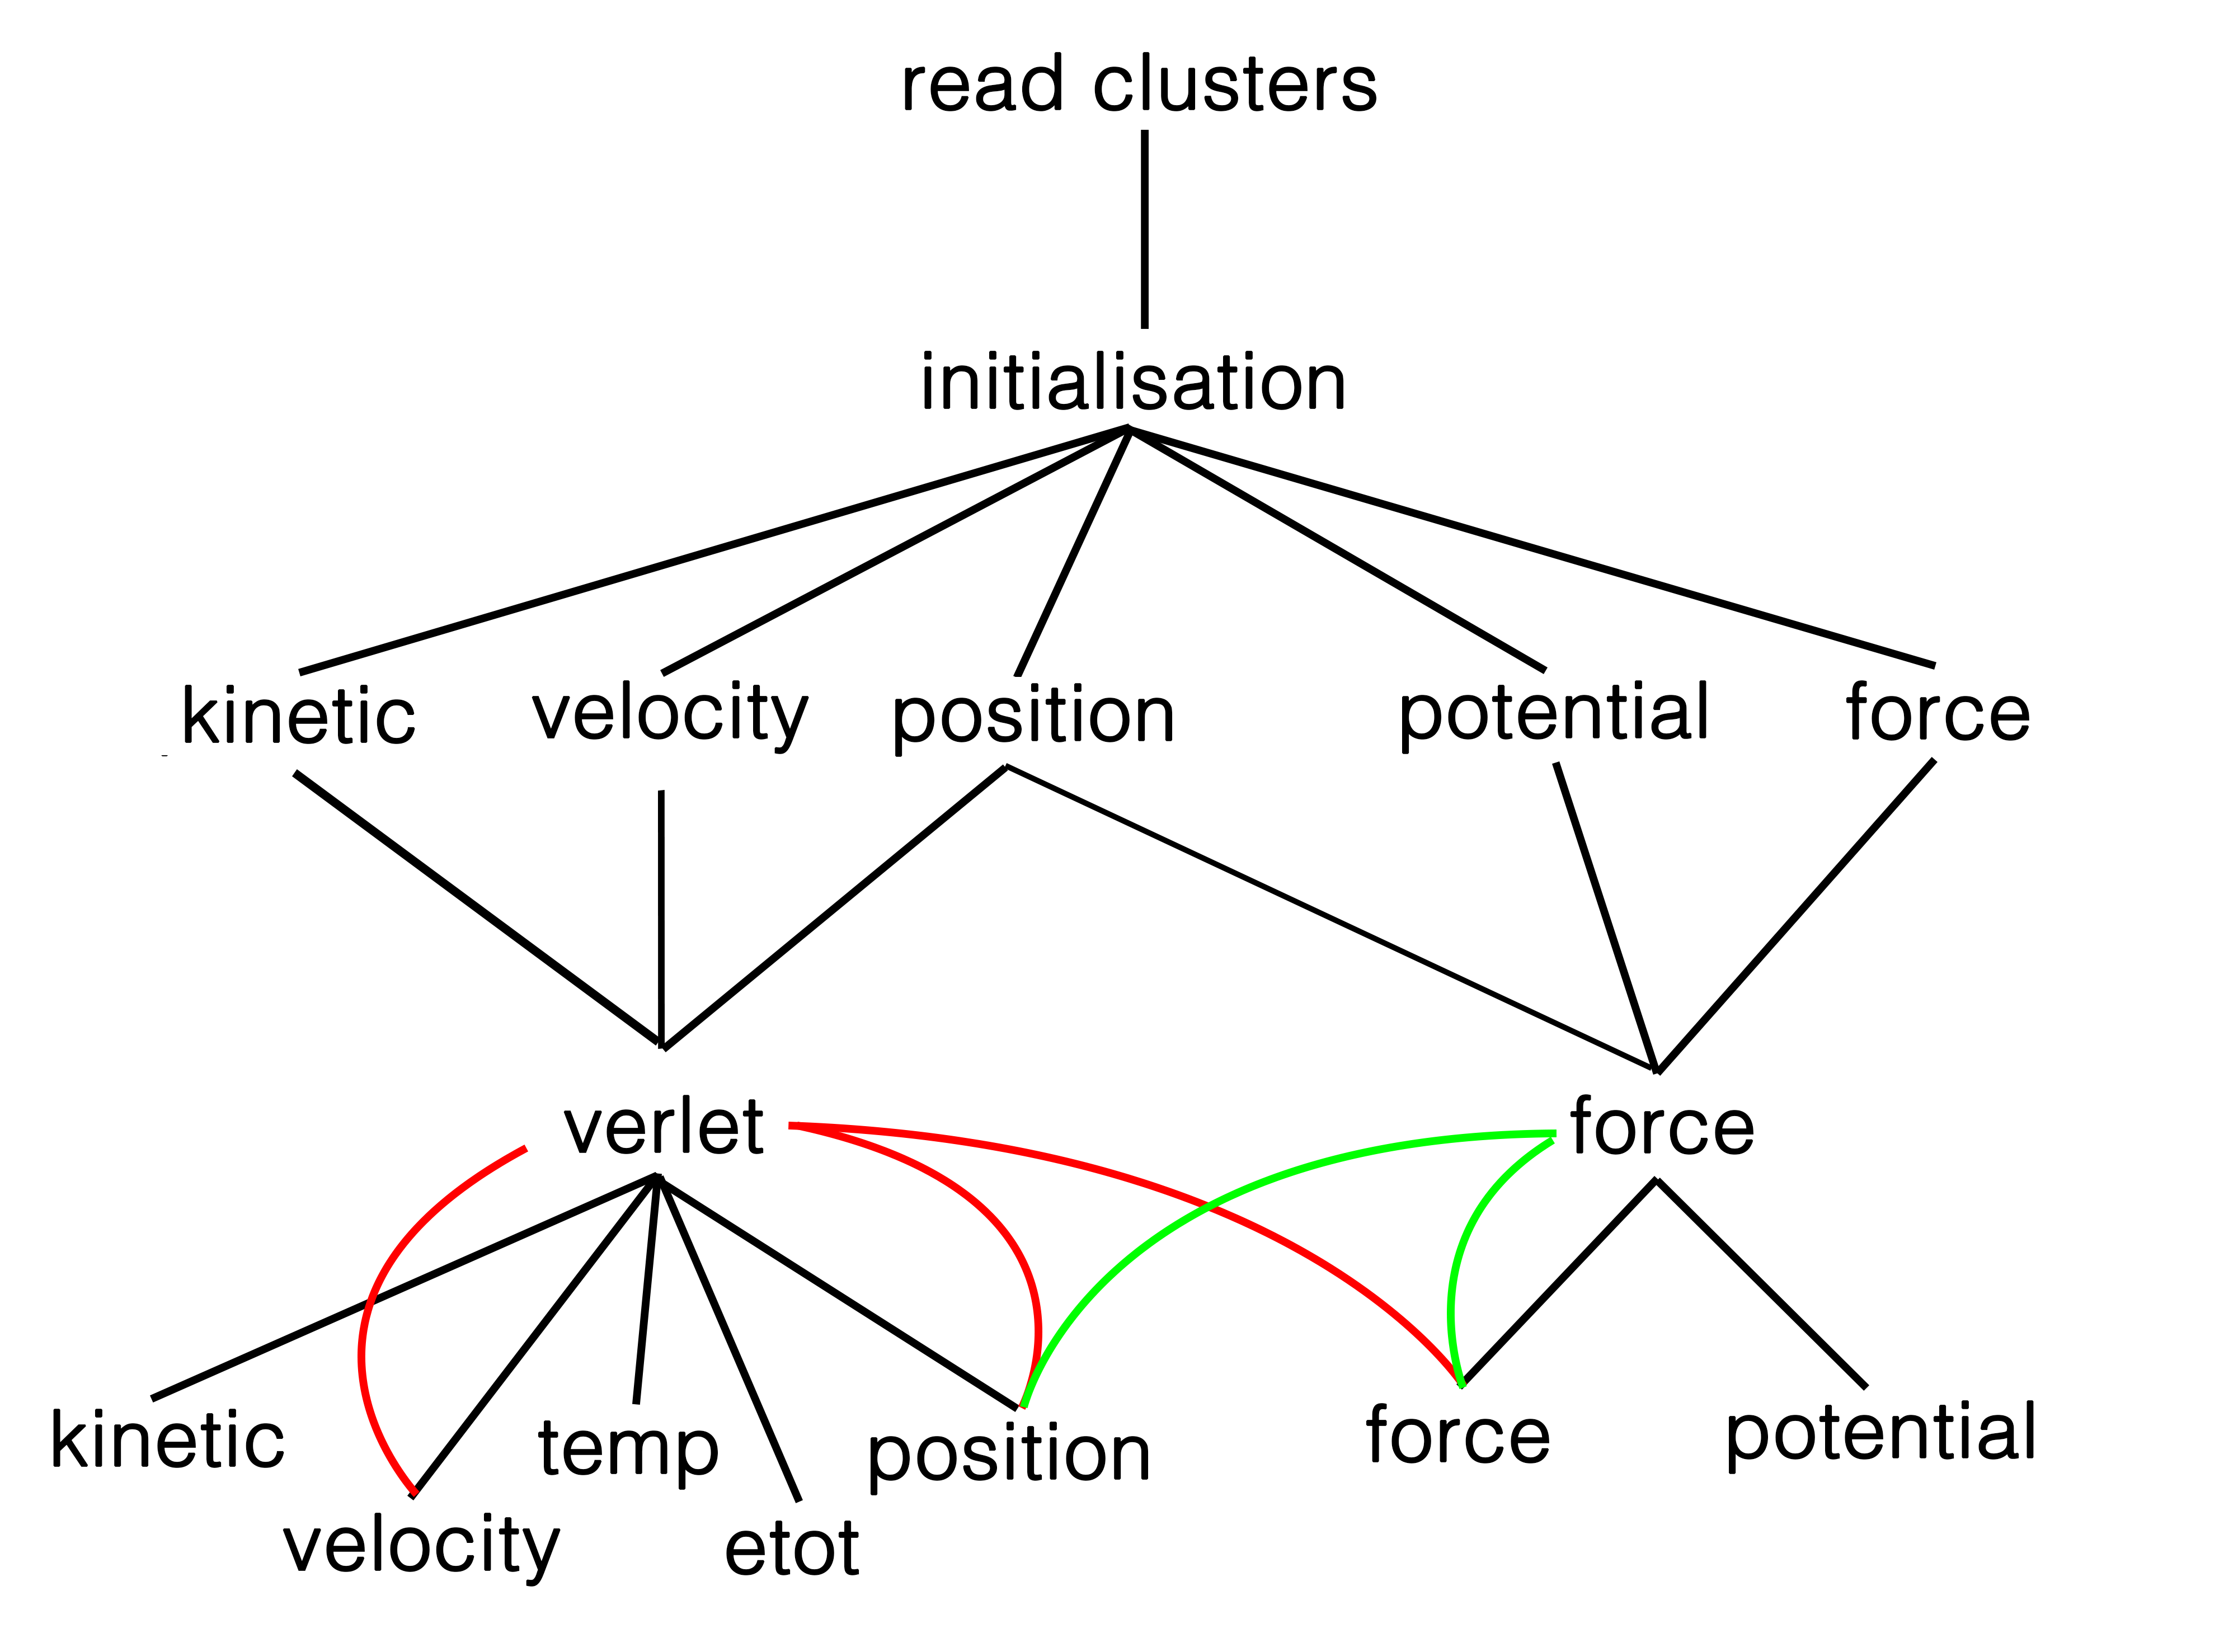
\includegraphics[width = 6.5cm]{tree_graph}} 

	
	The red and green curved connections represent the recursive nature of the program, wherein the outputs of a function are given as inputs at the next time-step, and hence the system evolved in time.


Additional, however inessential functions complete the first section of the code in: \textit{refold} and \textit{vel\_rescale}. The \textit{refold} function ensures that the particles remain within some defined bounds, and hence do not "escape" the concerned area of interaction. The \textit{vel\_rescale} function precludes a system "explosion", whereby the energy of the particles increases well above that desired. To remedy this problem the velocities are rescaled \cite{shell} \cite{frenkel} according to a rescaling factor of:\[\lambda = \sqrt{ \frac{T}{T_{inst}}}\]
where T is the desired system temperature and $T_{inst}$ the instantaneous system temperature. These two functions were found to be of use above certain limits of cluster speed or simulation time only.

	The second section of the code is concerned with the calling of the functions described above, and the output of final values to external files upon completion of the simulation. 
	
	At runtime the program first asks for input of the desired time-step size and number of steps for the simulation to be run, along with some recommended values. The \textit{get\_clusters} and \textit{init} functions are then called, and the clusters loaded into the program. A new matrix for storing the outputs is also constructed for writing per 1000 iterations. The core of the simulation can now begin, where for each time-step the \textit{get\_force} and \textit{verlet\_vel} functions are called, and the output values printed to the storage matrix. This process can be represented through the pseudo-code: 
	\captionsetup[lstlisting]{position=bottom,font=footnotesize}
\renewcommand{\lstlistingname}{Code}
\begin{lstlisting}
while t < deltat*Nsteps:
	call get_force()
	call verlet_vel()
	#update positions and forces
	pos = new_pos
	vel = new_vel
	force = new_force
	potential = new_potential
	#write values to storage
	if iter_number%1000 ==0:
		write temp,etot,kinetic,
				potential,time
	#increment iteration number and time
	iter_number = iter_number + 1
	t = t + deltat
\end{lstlisting}
\captionof{lstlisting}{Loop demonstrating calling of features}

The remainder of the code deals with the technicalities of saving the final cluster positions to a file named \textit{final\_state.xyz}, and the stored values of temperate, total energy per particle, kinetic energy, potential energy and time to a file named \textit{final\_values.txt}.
Furthermore, upon completion of the simulation the \textit{matplotlib} package will display a 3D plot of the initial and final cluster positions for comparison, as such:

\begin{center}
	
\renewcommand{\lstlistingname}{Figure}
	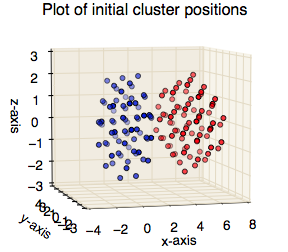
\includegraphics[width = 5cm,height=4cm]{init_cluster_pos} 
\captionbox[Text]{Plots of cluster position. \label{fig:dummy}}{
	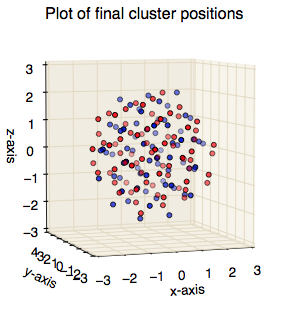
\includegraphics[width = 5cm,height=4.5cm]{final_cluster_pos}} 
\end{center}

To begin the simulation one must simply run the command:

\captionsetup[lstlisting]{position=bottom,font=footnotesize}
\renewcommand{\lstlistingname}{Code}
\begin{lstlisting}
>>python LJCollison.py
\end{lstlisting}
\setlength{\abovecaptionskip}{0pt plus 3pt minus 2pt}

\caption{Running the simulation from command line.}

in the directory of the file. The program simply requests input for the values of time-step, number of time steps, initial separation and initial velocity. The simulation, plotting and value writing is automated from hereon.

\onecolumn
\part{Collection of data}

The following pages are output and graphs of results from a simulation with input parameters:

\begin{center}
\begin{tabular}{ |c|c|c| } 
\hline
Parameter & Value \\
\hline
Time step & 1e-12 s\\ 
No. time steps & 50000 \\ 
Initial separation & 5\\ 
Initial velocity & 1e8\\
\hline
\end{tabular}
\end{center}
\end{multicols}
\begin{figure}[!h]
\center
\captionsetup{font=footnotesize,singlelinecheck=on}
\captionbox[Text]{Plots of initial and final cluster position automatically generated by the program. \label{fig:dummy}}{
	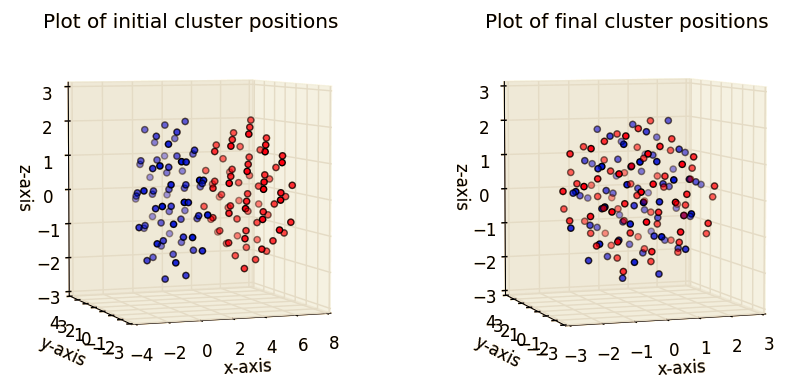
\includegraphics[width = 11cm,height=4.5cm]{output1}} 
\end{figure}
\captionsetup[lstlisting]{position=bottom,font=footnotesize}
\renewcommand{\lstlistingname}{Code}
\begin{lstlisting}
~~~~~~~~~~~~~~~~~~~~~~~~~~~~~~~~~~~~~~~~~~~~~~~~~~~~~
~~~~~~~~~~       SIMULATION COMPLETE       ~~~~~~~~~~

With  1e-12 s time-steps,  50000  steps, an
initial separation of  5.0  and an initial
velocity of  1e8 , the simulation took:  4648 s.

The final positions of the particles can be found in
the file final_state.xyz

The values, logged at every 1000 iterations can be
found in the file final_values.txt in the format:
________________________________________
| Temp  | E_tot   | E_kin  | E_pot |  Time   |
|------|--------|-------|-------|--------|
|       |         |        |        |        |

The matplotlib package should now be displaying a
plot of the initial and final cluster positions.

~~~~~~~~~~~~~~~~~~~~~~~~~~~~~~~~~~~~~~~~~~~~~~~~~~~~~
\end{lstlisting}
\captionof{lstlisting}{Output from program upon completion of simulation}
\renewcommand{\lstlistingname}{Table}
\pgfplotstableread{
1.757990867575163000e+15 2.619047619040545000e+15 3.849999999989607040e+17 -5.762554191765714222e+02 0.000000000000000000e+00
1.757990867575163000e+15 2.619047619040546000e+15 3.849999999989607040e+17 -4.263011298312022745e+02 1.000000000000003991e-09
1.757990867575163000e+15 2.619047619040552000e+15 3.849999999989607040e+17 4.497755364766907746e+02 2.000000000000075398e-09
1.757990867575163000e+15 2.619047619040595000e+15 3.849999999989607040e+17 6.787484430517741202e+03 2.999999999999968547e-09
1.757990867575163000e+15 2.619047619041002500e+15 3.849999999989607040e+17 6.670958527212130139e+04 3.999999999999975434e-09
1.757990867575163000e+15 2.619047619046257000e+15 3.849999999989607040e+17 8.391247045654669637e+05 5.000000000000282173e-09
1.757990867570803500e+15 2.619047619125921000e+15 3.849999999980059520e+17 1.350444526443661191e+07 6.000000000000588913e-09
1.757990867213250750e+15 2.619047619696225000e+15 3.849999999197018880e+17 1.756432230296096206e+08 7.000000000000895652e-09
1.757990865695338000e+15 2.619047621986943000e+15 3.849999995872790400e+17 8.448016289796568155e+08 8.000000000000748270e-09
1.757990820359031750e+15 2.619047689335506000e+15 3.849999896586279680e+17 2.067369138689103699e+10 9.000000000000227828e-09
1.757990772532919750e+15 2.619047761165293000e+15 3.849999791847094400e+17 4.170658857999176025e+10 9.999999999999707387e-09
1.757990864631898500e+15 2.619047623653907000e+15 3.849999993543857920e+17 1.322738569965136290e+09 1.099999999999918695e-08
1.757990867051347000e+15 2.619047620128023500e+15 3.849999998842449920e+17 2.745744726788842678e+08 1.199999999999866651e-08
1.757990866132905250e+15 2.619047621330674500e+15 3.849999996831062400e+17 6.525028840302489996e+08 1.299999999999814606e-08
1.757990864898992750e+15 2.619047623132431000e+15 3.849999994128794240e+17 1.187587877697824955e+09 1.399999999999762562e-08
1.757990867096481000e+15 2.619047619890387000e+15 3.849999998941293440e+17 2.297575831121544540e+08 1.499999999999726896e-08
1.757990858955762250e+15 2.619047632064016000e+15 3.849999981113119360e+17 3.802098434566435814e+09 1.599999999999840288e-08
1.757990783241756000e+15 2.619047745055504500e+15 3.849999815299445760e+17 3.699321457570290375e+10 1.699999999999953680e-08
1.757990851167500000e+15 2.619047643895523500e+15 3.849999964056824960e+17 7.246959446126844406e+09 1.800000000000067072e-08
1.757990861931475750e+15 2.619047627842825000e+15 3.849999987629932160e+17 2.529902079258154392e+09 1.900000000000180464e-08
1.757990861577039750e+15 2.619047628315009000e+15 3.849999986853717120e+17 2.676934592098865986e+09 2.000000000000293856e-08
1.757990859538677500e+15 2.619047631342588000e+15 3.849999982389703680e+17 3.568390069922412872e+09 2.100000000000407248e-08
1.757990866890718750e+15 2.619047620432020500e+15 3.849999998490673920e+17 3.544396139902586937e+08 2.200000000000520640e-08
1.757990867629023750e+15 2.619047619382943500e+15 3.850000000107562240e+17 3.853646702505104989e+07 2.300000000000634032e-08
1.757990867631051750e+15 2.619047619343679000e+15 3.850000000112003200e+17 3.232051911116363108e+07 2.400000000000747424e-08
1.757990867631203750e+15 2.619047619381044000e+15 3.850000000112336000e+17 3.777990904379828274e+07 2.500000000000860816e-08
1.757990867588833250e+15 2.619047619431131000e+15 3.850000000019544960e+17 5.442179106160715222e+07 2.600000000000974208e-08
1.757990867185552250e+15 2.619047619963432000e+15 3.849999999136359680e+17 2.209885324205379486e+08 2.700000000001087600e-08
1.757990866880708000e+15 2.619047620369975000e+15 3.849999998468750720e+17 3.475112278214636445e+08 2.800000000001200992e-08
1.757990865472264500e+15 2.619047622488785000e+15 3.849999995384259200e+17 9.674254591808642149e+08 2.900000000001314384e-08
1.757990866591115750e+15 2.619047620764532500e+15 3.849999997834543360e+17 4.689319473558268547e+08 3.000000000001427777e-08
1.757990867365979750e+15 2.619047619602183500e+15 3.849999999531495680e+17 1.283714091607111096e+08 3.100000000001541169e-08
1.757990867321766250e+15 2.619047619666651000e+15 3.849999999434668160e+17 1.475308965368737280e+08 3.200000000001654561e-08
1.757990867447684000e+15 2.619047619489803500e+15 3.849999999710428160e+17 9.395828859663522243e+07 3.300000000001767953e-08
1.757990867428347000e+15 2.619047619565838000e+15 3.849999999668080000e+17 1.093701530268884003e+08 3.400000000001881345e-08
1.757990852453242500e+15 2.619047641851100500e+15 3.849999966872600960e+17 6.664851696588201523e+09 3.500000000001994737e-08
1.757990406208577500e+15 2.619048306188927500e+15 3.849998989596784640e+17 2.020500939056053772e+11 3.600000000002108129e-08
1.757990800080776250e+15 2.619047720547022000e+15 3.849999852176899840e+17 2.970272223901868439e+10 3.700000000002221521e-08
1.757990691006226750e+15 2.619047882539203500e+15 3.849999613303636480e+17 7.740289925648219299e+10 3.800000000002334913e-08
1.757989776781040750e+15 2.619049235592464500e+15 3.849997611150479360e+17 4.765170443400886841e+11 3.900000000002448305e-08
1.757980441822551500e+15 2.619063201064965000e+15 3.849977167591387520e+17 4.573797411100983398e+12 4.000000000002561697e-08
1.757849544858771250e+15 2.619255731456065500e+15 3.849690503240709120e+17 6.154219997072776562e+13 4.100000000002675089e-08
1.757939715915952000e+15 2.618996234796919000e+15 3.849887977855934720e+17 3.648729553608671875e+12 4.200000000002788481e-08
1.757947994770680000e+15 2.618983776008343000e+15 3.849906108547789440e+17 4.218447517908797264e+09 4.300000000002901873e-08
1.757947926246184250e+15 2.618983877840509000e+15 3.849905958479143680e+17 3.419464041995648956e+10 4.400000000003015265e-08
1.757947783646599500e+15 2.618984091197975500e+15 3.849905646186053120e+17 9.678749708892471313e+10 4.500000000003128657e-08
1.757947556745887000e+15 2.618984424864241000e+15 3.849905149273492480e+17 1.955276941725173645e+11 4.600000000003242049e-08
1.757935517550900250e+15 2.619002396257486500e+15 3.849878783436471680e+17 5.473906203334674805e+12 4.700000000003355441e-08
1.757947582008815250e+15 2.618984390368609000e+15 3.849905204599305600e+17 1.849242549700532532e+11 4.800000000003468833e-08
1.757947989923502750e+15 2.618983781233294500e+15 3.849906097932471040e+17 6.048047187597882271e+09 4.900000000003582225e-08
}\datatable
\center
\pgfplotstabletypeset[
    columns/0/.style={
        column name=$Temperature$,
        dec sep align,
        /pgf/number format/fixed zerofill,
        /pgf/number format/precision=3
    },
    columns/1/.style={
        column name=$Total Energy$,  % ... and the second
        dec sep align,      % align on the decimal marker
        /pgf/number format/fixed zerofill,  % print trailing zeros
        /pgf/number format/precision=3     % print 14 digits
    },
    columns/2/.style={
        column name=$Kinetic Energy$,
        /pgf/number format/precision=3
    },
    columns/3/.style={
        column name=$Potential Energy$,
        /pgf/number format/fixed zerofill,
        /pgf/number format/precision=3
    },
       columns/4/.style={
        column name=$Time (s)$,
        dec sep align,
        /pgf/number format/precision=3
    },
    every head row/.style={
        before row=\toprule,    % booktabs rules
        after row=\midrule
    },
    every last row/.style={
        after row=\bottomrule
    }]{\datatable}


\caption{Output values from simulation.}
	\renewcommand{\lstlistingname}{Figure}
	\captionsetup{font=footnotesize,singlelinecheck=on}
\captionbox[Text]{VMD output from file \textit{final\_state.xyz}. \label{fig:dummy}}{
	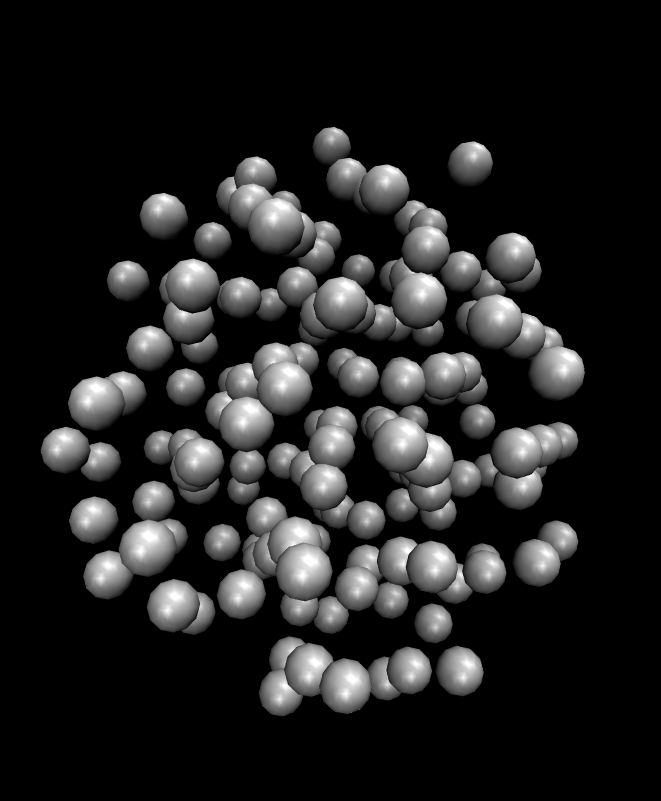
\includegraphics[height=4cm,width=4cm]{VMD}} 
\begin{center}
	
	\renewcommand{\lstlistingname}{Figure}
	\captionsetup{font=footnotesize,singlelinecheck=on}
\captionbox[Text]{Plot of Potential Energy vs Time. \label{fig:dummy}}{
	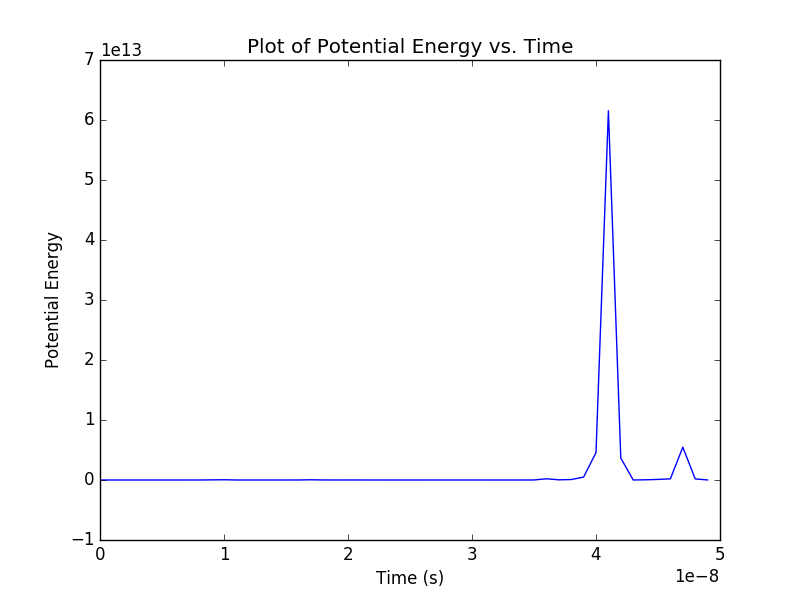
\includegraphics[height=5cm,width=6cm]{pot_time}} 
	\captionbox[Text]{Plot of Kinetic vs Time. \label{fig:dummy}}{
	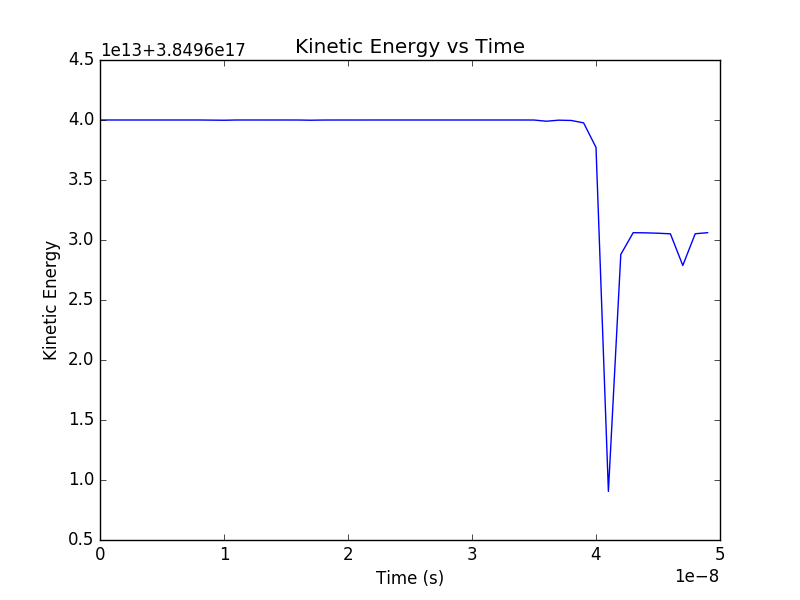
\includegraphics[height=5cm,width=6cm]{ekin}} 
\captionsetup{font=footnotesize,singlelinecheck=on}
\captionbox[Text]{Plot of Total Energy per particle vs Time. \label{fig:dummy}}{
	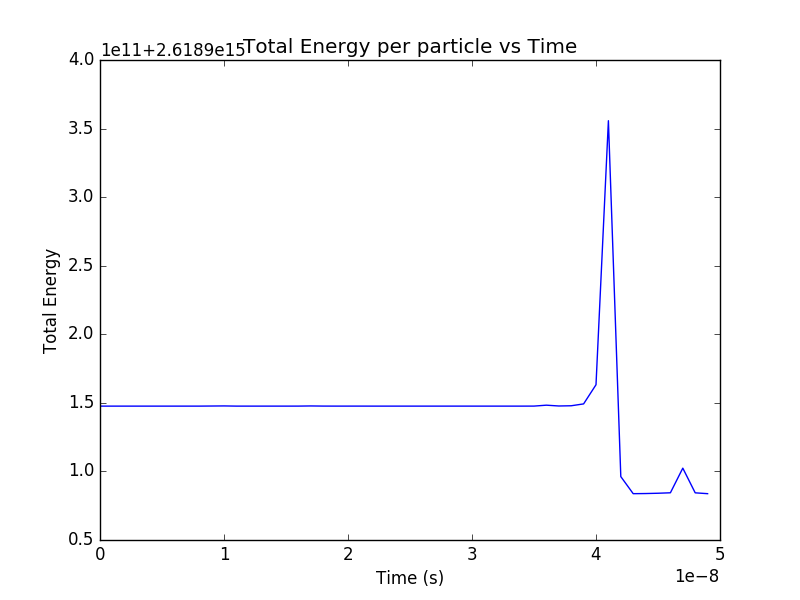
\includegraphics[height=5cm,width=6cm]{etot}} 
	
	\end{center}
	\begin{flushleft}
		
	
	As can be seen above, the two plots of energy follow a similar pattern. The initial peak around 40 nanoseconds represents the incoming cluster passing the cut-off radius, and hence a spike in the total energy per particle due to the introduction of the Lennard-Jones potential. This is the start of the coalescence process. The reduction in total energy per particle is caused by the drop in potential following this, and a corresponding increase in kinetic energy. There is once again a peak in potential energy, however the kinetic energy never returns to its initial value, resulting in an overall drop in total energy per particle.
	\end{flushleft}
\newpage
\twocolumn
\flushleft
\part{Conclusion}
A simple molecular dynamics program modelling the collision of two Lennard-Jones clusters was created and demonstrated using Python 3. The values of \textit{time-step size}, \textit{time-step number}, \textit{initial seperation} and \textit{initial velocity} are given to the program as user input, with the program initialising one cluster at the centre of the co-ordinate axes and the other travelling towards it. The Lennard-Jones potential was used to calculate the potential energy and force on the particles. The force calculation was then used in the Velocity Verlet algorithm to solve Newton's Equations of motion and evolve the system in time, and the equipartition theorem used to calculate the temperature of the system.  The calculated  vales of \textit{temperature}, \textit{total energy}, \textit{kinetic energy} and \textit{potential energy} are then printed to an output file, along with the final positions of the particles upon simulation completion. Initialisation values of:
\begin{center}
\begin{tabular}{ |c|c|c| } 
\hline
Parameter & Value \\
\hline
Time step & 1e-12 s\\ 
No. time steps & 50000 \\ 
Initial separation & 5\\ 
Initial velocity & 1e8\\
\hline
\end{tabular}
\end{center}

were found to successfully coalesce the two clusters within 50 nanoseconds.

\vspace{10cm}
\center
\begin{thebibliography}{9}
\bibitem{doye} 
Doye, Jonathan.
\textit{The Cambridge Cluster Database}
\\\texttt{http://doye.chem.ox.ac.uk/jon/}
\\\texttt{structures/LJ/tables.150.html}
(accessed December 12, 2016)

\bibitem{time-step} 
Franzen, Stefan. 
\textit{Introduction to Molecular Dynamics}. 
\\\texttt{http://www4.ncsu.edu/~franzen/}
\\\texttt{public\_html/CH795N/lecture/IV}
\\\texttt{/IV.html}
North Carolina State University (accessed December 12, 2016)
 
\bibitem{frenkel} 
Frenkel, Daan; Smit, Berend. 
\textit{Understanding Molecular Simulation: From Algorithms to Applications p.69}
Amsterdam: Elsevier Science, 2001. (accessed December 12, 2016)
 
\bibitem{ercolessi} 
Ercolessi, Furio.
\textit{Example code: example\_MD\_lj.f90}
SISSA, Trieste, May 1995

\bibitem{shell} 
Shell, M.S. 
\textit{Advanced Molecular Dynamics Techniques}. 
\\\texttt{https://engineering.ucsb.edu/}
\\\texttt{~shell/che210d/Advanced\_mole}
\\\texttt{cular\_dynamics.pdf}
University of California, Santa Barbara. (accessed December 12, 2016)

\end{thebibliography}
\newpage
\onecolumn
CODE APPENDIX
\lstinputlisting[language=Python]{LJCollision.py}
\end{document}